\documentclass[a4paper,10pt]{article}
\usepackage[spanish]{babel} % Paquetes de idioma
\usepackage[latin1]{inputenc} % Paquetes de idioma
\usepackage{graphicx} % Paquete para ingresar gráficos
\usepackage{grffile}
\usepackage{hyperref}
\usepackage{fancybox}
\usepackage{amsmath}
\usepackage{listings}

% Encabezado y Pié de página
\usepackage{fancyhdr} % Paquete para encabezados y pie de página
\pagestyle{fancy} % Sin esta línea no se imprimiría el encabezado en todas las páginas

\fancyhf{} %  Borra el encabezado anterior (Por defecto escribe el títutlo de la sección en la que se encuentra la hoja
\setlength{\headheight}{22.55pt}
\fancyhead[L]{
	{\textsf{Facultad de Ingenier\'ia $-$ Universidad de Buenos Aires \\ 75.59 T\'ecnicas de Programaci\'on Concurrentes I}}
}

\fancyhead[R]{\thepage}

\renewcommand{\footrulewidth}{0.4pt} % Ajusta el tamaño de las líneas separadoras en el pié de página
\renewcommand{\headrulewidth}{0.4pt} % Ajusta el tamaño de las líneas separadoras en el encabezado

\fancyfoot[L]{
	{\textsf{Trabajo Pr\'actico N$^{\circ}$1: ConcuShare}} \\
	{\textsf{Integrantes: Torres Feyuk, Hurtado, }}
	}
		

% Carátula del Trabajo
\title{ \author{} % Lo pongo para que el warning no moleste :p
\setlength{\unitlength}{1cm} %  Especifica la unidad de trabajo
\thispagestyle{empty}

\begin{picture}(18,0)
\put(0,0){
\includegraphics[width=1.5cm, height=3cm]{Logo1.png}}

\put(10.5,0){
\includegraphics[width=3cm, height=3cm]{Logo2.png}}

\end{picture}
\\[1.5cm]
\begin{center}
	\textbf{{\Huge Facultad de Ingenier\'ia \\ Universidad de Buenos Aires}}\\[2cm]
	{ 75.59 T\'ecnicas de Programaci\'on Concurrentes I}\\[0.5cm]
	{ Trabajo Pr\'actico N${^\circ}$1 : ConcuShare}\\[2.5cm]
\end{center}

\begin{flushleft}
	\textbf{Integrantes:} \\[1cm]

	\begin{tabular}{|c|c|c|}
		\hline
		\textbf{\normalsize Padr\'on} & \textbf{\normalsize Nombre} & \textbf{\normalsize Email} \\
		\hline
		\normalsize 87991 & \normalsize Ramonda, Juan Pablo & \normalsize juanpr@gmail.com \\
		\hline
		\normalsize 89542 & \normalsize Hurtado, Pablo Nicol\'as & \normalsize hurtado.pani@gmail.com \\
		\hline
		\normalsize 89579 & \normalsize Torres Feyuk, Nicol\'as R. Ezequiel & \normalsize ezequiel.torresfeyuk@gmail.com \\
		\hline
	\end{tabular}
\end{flushleft}
\date{} % Hace que no se imprima la fecha en la cual se compilo el .tex
 }

\begin{document}
	\maketitle % Hace que el título anterior sea el principal del documento
	\newpage

	\tableofcontents % Esta línea genera un indice a partir de las secciones y subsecciones creadas en el documento
	\newpage

	\section{Introducci\'on}
		El presente trabajo consiste en el desarrollo de una aplicaci\'on {\it concurrente} conocida como \emph{ConcuShare}. El objetivo de la misma
		es permitir el intercambio de archivos entre distintos usuarios. \\
		\indent Debido a que la materia apunta a obtener conocimientos sobre los mecanismos de concurrencia vistos hasta el momento en la c\'atedra, 
    el proyecto debe correr en una \'unica computadora y funcionar bajo un ambiente \emph{Unix/Linux} dado que los mecanismos vistos son los 
    implementados por \emph{System V}. \\
		\indent La implementaci\'on de la aplicaci\'on consiste en un esquema \emph{Cliente-Servidor}. El servidor se encuentra escuchando peticiones
		del cliente. Los clientes deben conectarse al servidor, y luego de esto pueden utilizar los servicios provistos por el mismo.
		\vspace{0.5cm}

	\section{Modo de Operaci\'on}

		\subsection {C\'omo compilar y correr la aplicaci\'on}
			Para poder correr la aplicaci\'on correctamente, lo primero que debe realizarse es compilar el programa. Para esto se ha provisto de un
			\emph{Makefile} que se encagar\'a de realizar el proceso de compilaci\'on. \\
			\indent Para compilar la aplicaci\'on servidor se debe ingresar el siguiente comando:
			\begin{verbatim}
				$ make server
			\end{verbatim}
			\indent Para compilar la aplicaci\'on cliente se debe ingresar el siguiente comando:
			\begin{verbatim}
				$ make client
			\end{verbatim}
			\indent Para compilar la aplicaci\'on que se encarga de realizar las transferencias, se debe ingresar el siguiente comando:
			\begin{verbatim}
				$ make transf
			\end{verbatim}
			\indent En el caso de que desee compilar todas las aplicaciones juntas puede hacerlo por medio de alguno de los siguientes comandos:
			\begin{verbatim}
				$ make server client transf
				$ make all
			\end{verbatim}

		Para correr la aplicaci\'on servidor o cliente en modo debug, se debe agregar el par\'ametro \emph{--debug} como se muestra a continuaci\'on:
		\begin{verbatim}
			$ ./server --debug
		\end{verbatim}

		\subsection{Casos de Uso}

			Como bien se dijo, la aplicaci\'on est\'a compuesta por un \emph{Servidor} que escucha peticiones y \emph{Clientes} que realizan las mismas. 
			De esta forma, el \emph{Servidor} es un proceso que no tiene interacci\'on con el usuario. En cambio, el \emph{Cliente} si tiene interacci\'on
			con el usuario. La aplicaci\'on \emph{Cliente} despliega un men\'u con las tareas que puede realizar el mismo. A continuaci\'on se 
			explica el modo de uso de cada una de las opciones del men\'u: 

			\begin{itemize}
				
                \item \textbf{1-Conectarse al Servidor:} Lo primero que debe hacer el cliente al iniciar la aplicaci\'on es conectarse a la misma. En el caso
				de no conectarse no podr\'a realizar ninguna otra tarea.
                
                Precondici\'on: El servidor se encuentra corriendo. El cliente se encuentra conectado.
                \begin{itemize}
                    \item El cliente solicita conectarse al servidor a trav\'es del canal de lectura del servidor.
                    \item El servidor recibe la solicitud y abre un canal de escritura para comunicarse con el cliente.
                \end{itemize}
                
                \item \textbf{2-Desconectarse del Servidor:} Si el cliente desea dejar la aplicaci\'on debe desconectarse del servidor. Al desconectarse, el
				servidor remueve de la lista de archivos compartidos todos los ficheros compartidos por este usuario.
                
                Precondici\'on: El servidor se encuentra corriendo. El cliente se encuentra conectado.
				\begin{itemize}
                    \item El cliente solicita al servidor desconectarse del mismo.
                    \item El servidor recibe el mensaje, cierra el canal de escritura por el cual se comunica con ese cliente y deja de compartir los archivos que compart\'ia el usuario dado de baja.
                \end{itemize}
                
                \item \textbf{3-Compartir Archivos:} Mediante esta opci\'on, el cliente le indica al servidor que archivos quiere disponer para ser compartidos.
				El mismo debe pasarle la ruta del archivo a compartir. La misma debe ser v\'alida.

                Precondici\'on: El servidor se encuentra corriendo. El cliente se encuentra conectado.
                \begin{itemize}
                    \item El usuario solicita compartir un archivo.
                    \item El programa cliente pregunta la ruta del archivo a compartir.
                    \item El usuario ingresa la ruta del archivo a compartir.
                    \item El programa cliente valida la ruta (E1) y la env\'ia al servidor.
                    \item El servidor agrega el archivo a la lista de archivos compartidos por el cliente correspondiente.
                \end{itemize}
                
                E1) La ruta no corresponde a un archivo existente.
                    \begin{itemize}
                        \item El programa cliente muestra un mensaje de error y vuelve al men\'u de selecci\'on de operaci\'on.
				    \end{itemize}
                
                \item \textbf{4-Descompartir Archivos:} Mediante esta opci\'on, el cliente le indica al servidor que archivos desea dejar de compatir con los 
				dem\'as usuarios. El mismo debe pasarle la ruta del archivo a descompartir, la cual debe ser v\'alida.
				
                
                Precondici\'on: El servidor se encuentra corriendo. El cliente se encuentra conectado. El cliente que solicita la baja del archivo compartido es el mismo que lo comparte.
                \begin{itemize}
                    \item El usuario solicita dejar de compartir un archivo.
                    \item El programa cliente pregunta la ruta del archivo a dejar de compartir.
                    \item El usuario ingresa la ruta.
                    \item El programa cliente verifica la existencia del archivo indicado (E1) y env\'ia un mensaje al servidor solicitando la eliminaci\'on del archivo de la lista de compartidos.
                    \item El servidor recibe el mensaje, elimina el archivo de la lista (E2) y responde con un mensaje de OK.
                    \item El cliente recibe el mensaje y notifica al usuario del \'exito de la operaci\'on.
                \end{itemize}

                E1) La ruta no corresponde a un archivo existente.
                \begin{itemize}
                    \item El programa cliente muestra un mensaje de error y vuelve al men\'u de selecci\'on de operaci\'on.
                \end{itemize}
                
                E2) Ocurri\'o un error en el servidor.
                \begin{itemize}
                    \item El servidor env\'ia un mensaje de error al cliente.
                    \item El cliente muestra un mensaje de error al usuario.
                \end{itemize}

                \item \textbf{5-Descargar Archivos:} Mediante esta opci\'on, el usuario puede elegir qu\'e archivos compartidos desea descargarse. Debe ingresar
				para esto el pid del cliente que se encuentra compartiendo el archivo, el path del archivo compartido y el path de destino.
				
                \begin{itemize}
			\item El usuario solicita transferir un archivo.
			\item El cliente pregunta el PID del cliente del cual se desea transferir el archivo.
			\item El usuario ingresa el PID.
			\item El cliente pregunta el path donde quiere descargar el archivo (debe ser un directorio).
			\item El usuario ingresa el path.
			\item El cliente pregunta el path del archivo compartido. Este se debe ingresar de la misma forma que est\'a en la lista de archivos compartidos.
			\item El usuario ingresa el path.
			\item El cliente verifica los paths, cancelando la operaci\'on en caso de error (E1) y mostrando el mensaje correspondiente
			\item Si todo est\'a bien, el cliente envia al servidor el comando para solicitar transferencia.
			\item El servidor crea el proceso \emph{Transferidor} pas\'andole los paths de origen y destino. Este ser\'a quien transmita el archivo.
			\item El servidor responde al cliente notific\'andole que todo est\'a listo para comenzar la transferencia.
			\item El cliente crea el proceso \emph{Transferidor} pas\'andole los paths. Este ser\'a quien reciba el archivo.
			\item Comienza la transferencia.
			\item Si todo sali\'o bien, el \emph{Transferidor} receptor notifica al usuario que la transferencia se ejecut\'o exitosamente.
                \end{itemize}
		E1) Errores posibles
		\begin{enumerate}
			\item El pid ingresado no es v\'alido (es 0).
			\item El path de destino no es v\'alido (quiz\'as no es un directorio).
			\item El path del archivo compartido no es v\'alido (puede no existir).
			\item El cliente con el PID ingresado no se encuentra conectado.
			\item El cliente ingresado no est\'a compartiendo el archivo especificado.
		\end{enumerate}
		\begin{itemize}
			\item El cliente muestra el mensaje de error correspondiente.
			\item El cliente vueve al men\'u principal.
		\end{itemize}

                \item \textbf{6-Obtener Lista de Archivos Compartidos:} Mediante esta opci\'on, el cliente obtiene la lista de los archivos compartidos por 
				todos los clientes que se encuentran conectados. La lista muestra los archivos compartidos por cada cliente, de modo que teniendo esta 
				informaci\'on se puede realizar la \emph{Descarga} de alg\'un archivo.
                   
                Precondici\'on: El servidor se encuentra corriendo. El cliente se encuentra conectado.
				
                \begin{itemize}
                   \item El usuario solicita al programa cliente que le muestre la lista de archivos compartidos.
                   \item El programa cliente solicita al servidor la lista de archivos compartidos.
                   \item El servidor env\'ia la lista.
                   \item El cliente recibe la lista y la muestra al usuario.
                \end{itemize}
                
                \item \textbf{7-Salir de la Aplicaci\'on:} Mediante esta opci\'on, el cliente abandona la aplicaci\'on.

                Precondici\'on: El servidor se encuentra corriendo. El cliente se encuentra conectado.
                
                \begin{itemize}
                    \item El usuario solicita salir del programa cliente.
                    \item Si el usuario se encuentra conectado, se desconecta.
                    \item Finaliza el programa cliente.
                \end{itemize}
			\end{itemize}

	\section{An\'alisis de la Soluci\'on}
		\subsection{Divisi\'on de la Aplicaci\'on en Procesos}
			Debido a la naturaleza de la soluci\'on adoptada, se pueden distinguir f\'acilmente los siguientes procesos:

			\begin{itemize}
				\item \textbf{Servidor:} Este proceso se encarga de escuchar las peticiones los clientes. Mientras ning\'un usuario le env\'ie ning\'un 
				mensaje, el mismo se bloquea. Cuando un cliente le env\'ia alg\'un mensaje, despierta al mismo y \'este se encarga de responderle al 
				usuario.
				\item \textbf{Cliente:} Al abrir un usuario una aplicaci\'on Cliente, se crea un nuevo proceso el cual puede comunicarse con el servidor.
				El Cliente env\'ia peticiones al servidor esperando una respuesta del mismo.
				\item \textbf{Transferidor:} Este proceso se crea cada vez que un cliente desea descargarse un archivo compartido. Tanto el Servidor como
				el Cliente crean un proceso \emph{Transferidor} por el cual se comunican para realizar la transferencia.
			\end{itemize}

		\subsection{Comunicaci\'on entre Procesos}
			A continuaci\'on se detalla como es la comunicaci\'on entre los procesos que componen a \emph{ConcuShare}, seg\'un los casos de uso:
			\begin{itemize}
				\item \textbf{Alta:}	
					\begin{itemize}
						\item El servidor y un cliente se comunican.
						\item El cliente env\'ia un mensaje al servidor pidiendo conectarse.
						\item El servidor da de alta al cliente en el caso de que no est\'e conectado. Informa esto por medio de 
									otro mensaje.
					\end{itemize}
				\item \textbf{Baja:}	
					\begin{itemize}
						\item El servidor y un cliente se comunican.
						\item El cliente env\'ia un mensaje al servidor pidiendo desconectarse.
						\item El servidor da de baja al cliente en caso de que no est\'e conectado. Informa esto por medio de
									otro mensaje.
					\end{itemize}
				\item \textbf{Compartir Archivo:}	
					\begin{itemize}
						\item El servidor y un cliente se comunican.
						\item El cliente env\'ia un mensaje al servidor para compartir un archivo.
						\item El servidor recibe el mensaje y contesta al cliente pidiendo el path completo del
									archivo a compartir.
						\item El cliente env\'ia el path al servidor y este lo almacena en la lista de compartidos. 
					\end{itemize}
				\item \textbf{Descompartir Archivo:} 
					\begin{itemize}
						\item El servidor y un cliente se comunican.
						\item El cliente env\'ia un mensaje al servidor para descompartir un archivo.
						\item El servidor recibe el mensaje y contesta al cliente pidiendo el path completo del
								archivo a descompartir.
						\item El cliente env\'ia el path al servidor y este elimina al mismo de su lista de compartidos
								si es que el usuario estaba compartiendo ese archivo.
					\end{itemize}
				\item \textbf{Descargar Archivo:}
					\begin{itemize}
						\item El servidor y un cliente se comunican a trav\'es del proceso Transferidor.
						\item El cliente env\'ia un mensaje al servidor pidiendo descargar un archivo.
						\item El servidor recibe el mensaje y contesta al cliente pidiendo el path completo del 
									archivo a descargar, el pid del cliente que posee el archivo y un path de destino
									donde almacenar el archivo.
						\item El cliente env\'ia esta informaci\'on al servidor y llama al proceso Transferidor para
									recibir el archivo.
						\item El servidor recibe la informaci\'on del cliente y llama al proceso Transferidor para
									enviar el archivo.
						\item El proceso Transferidor se encarga de transferir el archivo y al terminar esta operaci\'ion 
									informa y al servidor y al cliente el estado de la misma.
					\end{itemize}
				
				\item \textbf{Obtener Lista de Archivos Compartidos:}
					\begin{itemize}
						\item El servidor y un cliente se comunican.
						\item El cliente env\'ia un mensaje al servidor pidi\'endole la lista de archivos compartidos.
						\item El servidor le responde envi\'andole la lista de archivos compartidos serializada.
					\end{itemize}
			\end{itemize}

	\subsection{Problemas Conocidos de Concurrencia en el Trabajo}
	Respecto a las transferencias, como se mencion\'o, utilizan Memoria Compartida. Se podr\'ia comparar con el 
	problema de \emph{Consumidor Productor}, con la excepci\'on de que habr\'ia un solo consumidor y un solo productor. \\
	Sin embargo, se tienen los mismos problemas que en el modelo, ya que el lector debe esperar a que el escritor
	 ``produzca'' 
	y el escritor debe esperar a que el lector ``consuma''.
	
	Respecto a la comunicaci\'on entre cliente y servidor, se utiliza una FIFO para que el servidor lea los comandos de 
	todos los clientes. La comunicaci\'on tambi\'en se parece al problema de \emph{Cosumidor Productor},
	 con la
	 excepci\'on de que puede haber muchos productores y un solo consumidor. En el caso de las respuestas del servidor
	 a cada
	 cliente, se utiliza una FIFO para cada uno. Aqu\'i, solo hay un productor y un consumidor.\\
	En este caso, el lector siempre debe esperar a que el escritor ``produzca''.

	Respecto a la lectura del archivo para la transferencia, se podr\'ia comparar con el modelo de \emph{Lectores
	 Escritores}, aunque en la aplicaci\'on se pueden tener varios lectores para el archivo a transferir
	y un solo escritor para el archivo nuevo. \\Aunque, an\'alogamente 
	al caso anterior, se pueden presentar los problemas caracter\'isticos de este modelo, es decir, podr\'ia darse el caso
	de que se desee modificar de forma externa al archivo de lectura mientras est\'a siendo leido. Para el archivo de 
	escritura, 
	podr\'ia ser que se quiera leer o escribir el archivo mientras se est\'a escribiendo. 
	Para resolver estos problemas, se utilizan
	 Locks para los archivos en cuesti\'on.

	\subsection{Mecanismos de Concurrencia Utilizados}
		A continuaci\'on se exhiben los mecanismos de concurrencia utilizados en la comunicaci\'on entre los procesos:
		\subsubsection{Env\'io de Mensajes entre Servidor y Cliente}
			Los clientes se comunican con el servidor enviando mensajes con la tarea que desean realizar. Dado que el servidor 
			debe responder al cliente sobre el estado de la operaci\'on realizada, los mecanismos posibles para establecer esta 
			comunicaci\'on podr\'ian ser \emph{Fifos} o \emph{Memoria Compartida}. No se podr\'ia haber utilizado \emph{pipes} dado 
			que el cliente deber\'ia ser hijo del servidor, cosa que no ocurre. \\
			\indent Se decidi\'o utilizar \emph{Fifos} para establecer esta comunicaci\'on dado que los mensajes que env\'ia el cliente
			tienen distintos tama\~nos seg\'un la tarea a realizar, y en algunos casos como a la hora de compartir archivos, var\'ian 
			seg\'un la longitud del path del archivo compartido. \\ \\
			\indent De esta forma, el servidor posee una \emph{Fifo} para recibir mensajes del cliente y cada cliente posee una \emph{Fifo}
			para escribir mensajes al servidor. Con esta implementaci\'on surge un inconveniente: Una \emph{Fifo} es un mecanismo de 
			concurrencia unidireccional que asegura el sincronismo entre procesos. Sin embargo, dado que todos los clientes conectados poseen
			la \emph{Fifo} de lectura del servidor abierta, ya no existe sincronismo entre los procesos.  \\
			\indent Para solucionar este problema, se agrega un sem\'aforo. Este sem\'aforo se encarga de bloquear al servidor mientras que no 
			haya alg\'un cliente que intente escribir alg\'un mensaje. El cliente que desea escribir un mensaje incrementa el sem\'aforo y 
			despierta al servidor para procesar el mensaje. \\ \\
			\indent Los mensajes que el servidor env\'ia a cada cliente son entregados tambi\'en por medio de \emph{Fifos}. En este caso, el 
			servidor posee una \emph{Fifo} por cada cliente que se encuentre conectado, por lo cual no existen problemas de sincronismo dado que
			este mecanismo s\'olo es compartido entre el servidor y un cliente particular.

			\subsubsection{Transferencia de Archivos}
			Para realizar la transferencia de archivos se pod\'ia elegir nuevamente entre \emph{Fifos} y \emph{Memoria Compartida}. En este caso,
			se eligi\'o el mecanismo de concurrencia de \emph{Memoria Compartida}. El motivo de esta elecci\'on es que de esta forma el archivo
			compartido se escribe en memoria y no en un archivo en disco como se lo hace utilizando \emph{Fifos}. De esta forma, se mejora el 
			rendimiento de la aplicaci\'on. \\
			\indent Dado que el tama\~no del archivo puede llegar a ser muy grande, el archivo se escribe de forma particionada en la 
			\emph{Memoria Compartida}. \\
			\indent Para asegurar la sincronizaci\'on entre escrituras y lecturas, se emplean dos sem\'aforos. Un sem\'aforo bloquea 
			la lectura de la \emph{Memoria}. Esto se requiere en caso de que otro proceso se encuentre escribiendo la misma. Al terminar
			de escribir, el proceso desbloquea la \emph{Memoria Compartida} y el proceso que deseaba realizar una lectura se libera para
			poder completarla. El otro sem\'aforo bloquea la escritura de la \emph{Memoria}. Esto se requiere en caso de que un proceso
			se encuentre leyendo la memoria a la hora de que otro quiera escribirla. En este caso, el proceso que escribe se suspende 
			hasta que el proceso que lee incremente el sem\'aforo, lo cual se da cuando termina de leer.
			

			\subsubsection{Escritura sobre el Logger} 
				Al ejecutarse la aplicaci\'on en \emph{Modo Debug}, muchos procesos podr\'ian escribir el archivo al mismo tiempo. Esto
			puede provocar que los mensajes se mezclen entre s\'i y el archivo de log quede ilegible.
			Para solucionar este inconveniente, se agrega un lock de escritura sobre el archivo de log cada vez que un proceso logea
			alg\'un mensaje. El mismo se retira al terminarse la escritura sobre el mismo, dejando que cualquier otro proceso pueda 
			escribir otro mensaje.

	\section{Diagramas}
		
		\subsection{Diagramas de Estado}
			\begin{figure}[!htpb]
				\centering
				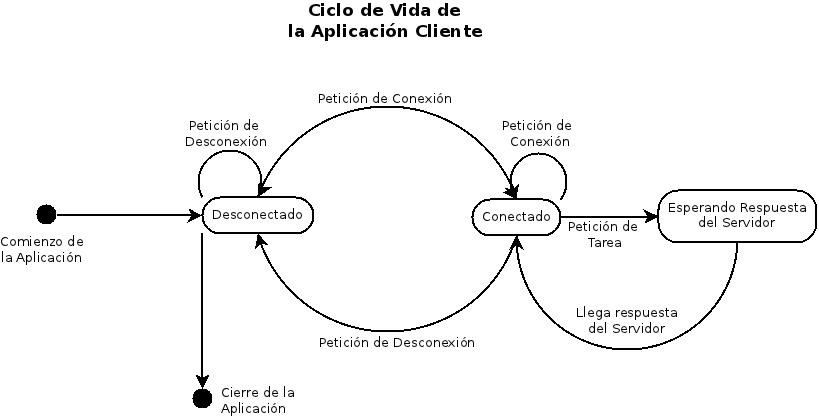
\includegraphics[width=12cm]{DEstadoVidaCliente.jpeg}
				\caption{Diagrama de Estado del Proceso Cliente} \label{Img001}
			\end{figure}

			\begin{figure}[!htpb]
				\centering
				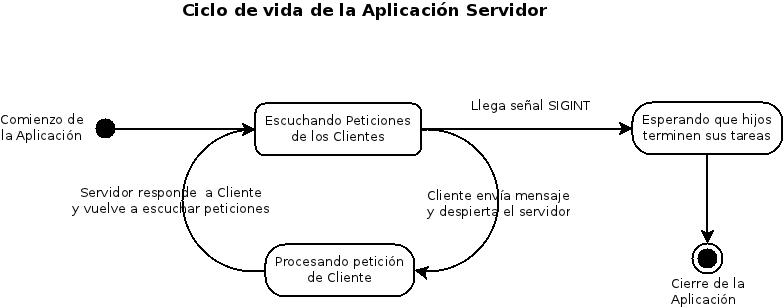
\includegraphics[width=12cm]{DEstadoVidaServidor.jpeg}
				\caption{Diagrama de Estado del Proceso Servidor} \label{Img002}
			\end{figure}

		\newpage
		\subsection{Diagrama de Clases}
			\begin{figure}[!htpb]
				\centering
				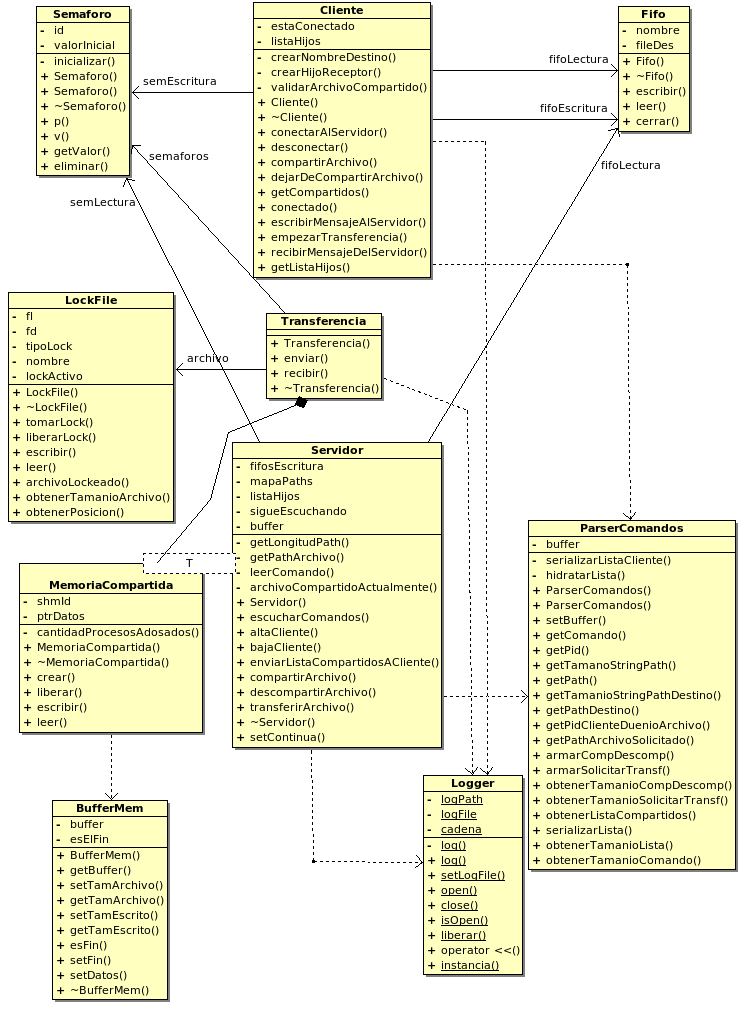
\includegraphics[width=12cm]{dclases.png}
				\caption{Diagrama de Clases de la Aplicaci\'on ConcuShare} \label{Img001}
			\end{figure}
		
			
			
		
		

				
\end{document}
